\documentclass[a4paper,twocolumn]{article}

\usepackage{times}
\usepackage[utf8]{inputenc}
\usepackage[portuguese, english]{babel}
\usepackage[a4paper,margin=2cm,columnsep=1cm]{geometry}
\usepackage{authblk}
\usepackage{titlesec}
\usepackage[pdftex]{graphicx}
\usepackage{mathtools}


\begin{document}

\graphicspath{{images/}}
\renewcommand{\abstractname}{\normalsize\bfseries\filcenter ABSTRACT}
\titleformat*{\section}{\normalsize\bfseries\filcenter}
\titleformat*{\subsection}{\small\bfseries\filcenter}
\renewcommand{\refname}{\normalsize\bfseries\filcenter REFERÊNCIAS}
\renewcommand{\figurename}{\small Figura}
\newcommand{\figureref}[1]{\textit{Figura \ref{fig:#1}}}
\newcommand{\equationref}[1]{\textit{Equação \ref{eq:#1}}}
\newcommand{\bigsum}{\displaystyle\sum}

\title{\textbf{Modulações Digitais BPSK e QPSK}}
\author{\textit{Eduardo M. B. de A. Tenório\textsuperscript{1}, Diogo B. da Silva\textsuperscript{2}, Gilberto P. de F. Sobrinho\textsuperscript{2}, Rodrigo J. C. Q. Peixe\textsuperscript{3} e Daniel C. Cunha\textsuperscript{1}}}
\affil{Centro de Informática, Universidade Federal de Pernambuco\\
Recife, PE, Brasil -- www.cin.ufpe.br\\
\small\textsuperscript{1}\texttt{\{embat,dcunha\}@cin.ufpe.br}\\
\small\textsuperscript{2}\texttt{\{diogo.bs1,gibapfarias\}@hotmail.com}\\
\small\textsuperscript{3}\texttt{rodrigo.peixe@gmail.com}}
\date{Agosto, 2014}

\maketitle

\begin{abstract}
\begin{itshape}
Colocar abstract aqui.

\noindent\textbf{palavras-chave}: modulação digital, bpsk, qpsk, AWGN, Rayleigh
\end{itshape}
\end{abstract}


\section{INTRODUÇÃO}

Este projeto teve como objetivo a implementação de uma simulação computacional de sistemas de comunicação digitais, utilizando as modulações Phase-Shift Keying (PSK) e Quadrature Amplitude Modulation (QAM). A forma de avaliar o desempenho de cada tipo de modulação foi através da taxa de erro de bit versus a relação sinal-ruído. Foi efetuada uma comparação dos desempenhos da curva analítica e da curva simulada, utilizando um canal com Ruído Aditivo Gaussiano Branco (AWGN) e Desvanecimento Rayleigh.

As modulações especificadas foram a BPSK (2-PSK) e QPSK (4-PSK), subtipos da modulação PSK, e 16-QAM e 64-QAM, subtipos da modulação QAM. O empreendimento obteve sucesso parcial, com a implementação da simulação para as modulações do tipo M-PSK, a adição do AWGN e o Desvanecimento Rayleigh.

O restante do documento está organizado da seguinte forma: na seção 2 há um descrição sucinta do AWGN. O Desvanecimento Rayleigh é descrito na seção 3. A seção 4 fala sobre a modulação PSK, detalhando a BPSK e a QPSK. Na seção 5 é descrita a simulação. A seção 6 apresenta a conclusão do trabalho e, por fim, as referências.

Todo o código utilizado para este trabalho, bem como imagens e demais documentos (este incluso) encontram-se num repositório no Github, disponível através da url \textit{https://github.com/embatbr/psk-qam}. A linguagem utilizada foi Python, versão 3.4.


\section{ADDITIVE WHITE GAUSSIAN NOISE}

Ruído é um sinal de natureza aleatória que interfere no sinal transmitido, algumas vezes ocasionando uma diferença na detecção da mensagem (no caso de uma mensagem binária, por exemplo, alguns bits podem ser trocados durante a transmissão), o que é considerado um erro. Uma forma de saber o quão resistente a ruídos é um sinal é a relação sinal-ruído (SNR, de \textit{signal-to-noise ratio}), que nada mais é que uma razão entre a potência do sinal enviado e a potência do ruído.

O AWGN é um ruído aditivo (ou seja, seu valor é adicionado ao valor do sinal), branco (todas as faixas de frequência possuem a mesma potência) e cuja amplitude segue uma distribuição gaussiana (distribuição normal). O termo ``ruído branco" é derivado do conceito de luz branca, que existe em todo o espectro de frequência. O ruído é dado pela equação

\begin{equation}
    n(x) = \frac{1}{\sigma \sqrt{2\pi}} e^{- \frac{(x - \mu)^2}{2\sigma^2}}
\end{equation}

\noindent com $\mu = 0$ e $\sigma^2 = \frac{N_0}{2}$. O sinal recebido é dado por $y(t) = s(t) + n(t)$, onde $s(t)$ é o sinal transmitido e $n(t)$ é o ruído.

A probabilidade de erro de bit, $P_b$ de um sinal em um canal com AWGN é dada pela equação abaixo. Para cada valor de SNR, o valor correspondente do Bit Error Rate (BER) é o $P_b$.

\begin{equation}
    \label{eq:prob_bit}
    P_b = \frac{1}{2}erfc(\sqrt{\frac{E_b}{N_0}})
\end{equation}


\section{DESVANECIMENTO RAYLEIGH}

Modelo estocástico de propagação no ambiente de um sinal de rádio, que ocorre quando não há ``visão" direta entre a fonte e o receptor. Como a propagação é indireta, o sinal apresenta um decaimento (desvanecimento) devido à reflexão, que varia aleatoriamente, de acordo com a distribuição Rayleigh, descrita pela equação

\begin{equation}
    p(h) = \frac{h}{\sigma^2}e^\frac{-h^2}{2\sigma^2}
\end{equation}

A probabilidade de erro de bit num canal com AWGN e Desvanecimento Rayleigh é dada pela equação a seguir, derivada da \equationref{prob_bit}.

\begin{equation}
    P_b = \frac{1}{2}(1 - \sqrt{\frac{\frac{E_b}{N_0}}{\frac{E_b}{N_0} + 1}})
\end{equation}


\section{MODULAÇÃO PSK}

Phase-shift keying (ou \textit{chaveamento por descolamento de fase}) é um esquema de modulação digital que atua alterando a fase da onda portadora (vide figura abaixo).

\begin{figure}[h]
    \label{fig:psk_mod}
    \centering
    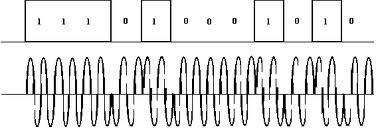
\includegraphics[scale=0.55]{psk-mod}
    \caption{\textit{Modulação PSK. Veja como a fase da portadora muda ao trocar o bit.}}
\end{figure}

Comumente é chamado de modulação M-PSK, onde M indica o número de símbolos (2, 4, 8\dots). As duas modulações estudadas para este projeto foram a binary phase-shift keying (BPSK) e a quadrature phase-shift keying (QPSK), ambas descritas nas subseções a seguir.

\subsection{BPSK}

A BPSK ou 2-PSK

\subsection{QPSK}


\section{SIMULAÇÃO}


\section{CONCLUSÃO}


\begin{thebibliography}{9}
    \bibitem{sklar_book}
        B. Sklar,
        ``Fading Channels,"
        in \textit{Digital Communications: Fundamentals and Applications,}
        2nd ed.
        Tarzana, California: University of California, Los Angeles,
        2001, ch. 15, pp. 944-1011.

    \bibitem{comm_theory}
        http://wiki.scipy.org/Cookbook/CommTheory

    \bibitem{dsplog_1}
        http://www.dsplog.com/2007/08/05/bit-error-probability-for-bpsk-modulation/

    \bibitem{dsplog_2}
        http://www.dsplog.com/2008/08/10/ber-bpsk-rayleigh-channel/
\end{thebibliography}

\end{document}